Using 
	  \eqref{eq:section_formula},
the mid point coordinates are given by
	\begin{align}
		\vec{P} = \frac{1}{2}\vec(\vec{A}+\vec{B})  = \myvec{1\\0}\\
		\vec{Q} = \frac{1}{2}\vec(\vec{B}+\vec{C}) = \myvec{1\\2}\\
		\vec{R} = \frac{1}{2}\vec(\vec{A}+\vec{C}) = \myvec{0\\1}
	\end{align}
	\begin{align}
\because		\vec{P}-\vec{Q} =  \myvec{
 0 \\
 -2 
 },\,
		\vec{Q}-\vec{R} =   \myvec{
 1 \\
 1 
 }
 \\
		ar(PQR)=\frac{1}{2}{\norm{\vec(\vec{P}-\vec{Q})\times\vec(\vec{Q}-\vec{R})}}
		=1
	\end{align}
	Similarly, 
	\begin{align}
		\vec{A}-\vec{B} = \myvec{
 -2 \\
 -2 
 }
 ,\,
		\vec{A}-\vec{C} =  \myvec{
 0 \\
 -4 
 }
 \\
 \implies
		ar(ABC)=\frac{1}{2}{\norm{\vec(\vec{A}-\vec{B})\times\vec(\vec{A}-\vec{C})}}
=4
\\
		\implies \frac{ar\brak{PQR}}{ar\brak{ABC}} = \frac{1}{4}
	\end{align}
	See 
\figref{fig:10/7/3/3Fig}
\begin{figure}[H]
	\begin{center} 
	    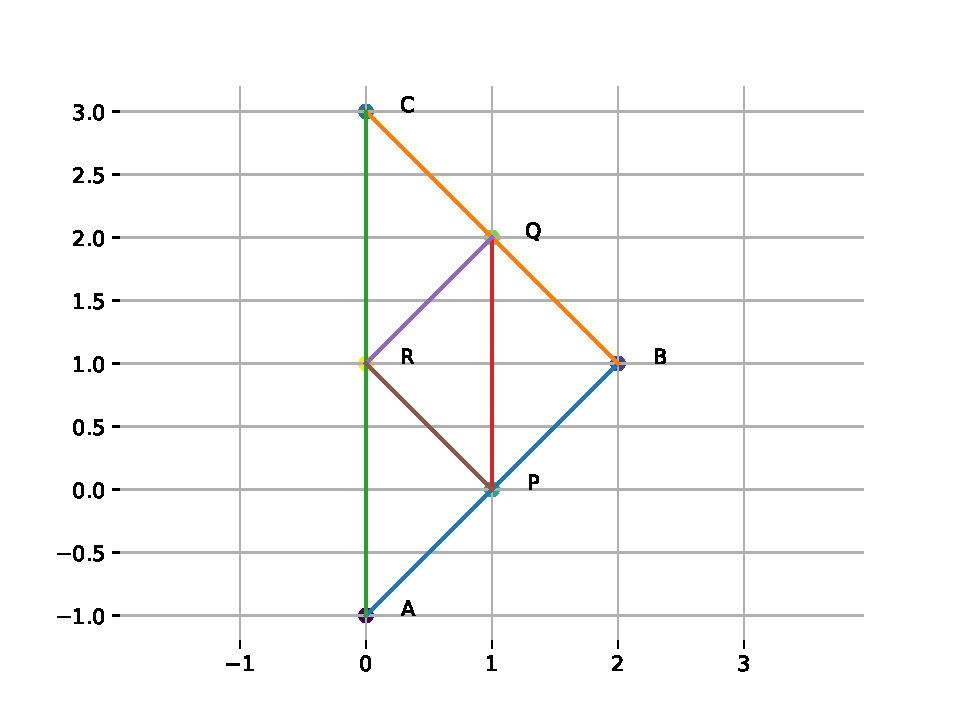
\includegraphics[width=0.75\columnwidth]{chapters/10/7/3/3/figs/fig.pdf}
	\end{center}
\caption{}
\label{fig:10/7/3/3Fig}
\end{figure}
